\section{Method}
\paragraph{Overview}
\begin{itemize}
\item compute medial axis transform (MAT)
\item find verts `of high curvature' in the medial axis
\item round the distance measures at those locations to integer multiples of the middle of the range of possible bead widths
\item introduce points on the `arms' of the medial axis connected to the changed verts, around even subdivision of the distance measures
\item connect points to the outline with new fingers
\item introduce new locations on the `fingers' of the medial axis at ideas distances for fingers from non-rounded medial axis verts
\item introduce new locations on the fingers at regular intervals for medial axis verts with rounded distance measures
\item connect all locations to form the inset polygons and polylines
\end{itemize}


\subsection{Straight Skeleton or Medial Axis?}
Medial Axis!
Medial axis is stable against small perturbations in the input polygon!
Concave corners are handled irrespective of how many vertices are in a corner.


$\to$ approximate parabolas for simpler processing!

This approximation leads to even spacing,
while a derived formula seems to produce different results:

See \url{/home/t.kuipers/Documents/PhD/Variable_Width_project/pathplanning preliminaries/medial_axis_parabolas.svg}

\Cref{medial_axis_parabolas}

\begin{figure}[H]
\begin{subfigure}{0.9\columnwidth}
\includegraphics[width=\columnwidth]{sources/method/medial_axis_even_spacing.jpg}
\caption{Parabola transformed to straight skeleton and offsets using even spacing along bones.}
\end{subfigure}
\begin{subfigure}{0.9\columnwidth}
\includegraphics[width=\columnwidth]{sources/method/medial_axis_uneven_spacing.pdf}
\caption{Parabola function plots from analytical solutions where the distance to the point is a whole fraction of the distance to the line.}
\label{medial_axis_parabolas_functions}
\end{subfigure}
\caption{The equidistant points between a vert and a line form a parabola. There are different methods for generating toolpaths which are in between the medial axis and the outline. Note that the uneven spacing does \emph{not} coincide with an even angular spacingat the border between the patches: see the left side of \subref{medial_axis_parabolas_functions}.}
\label{medial_axis_parabolas}
\end{figure}

\hl{But the uneven spacing figure looks like its evenly spaced in the direction orthogonal to the toolpath itself!}

Perhaps we should not space the joints evenly along the bones, but make the spacing depend on the angles involved.
We could check the intersection point of the lines of two polygon segments and radially project lines with the same angular spacing.
No, the angular spacing for two patches connected to a single bone would be different, so the paths wouldn't connect!

\begin{figure}[H]
\centering
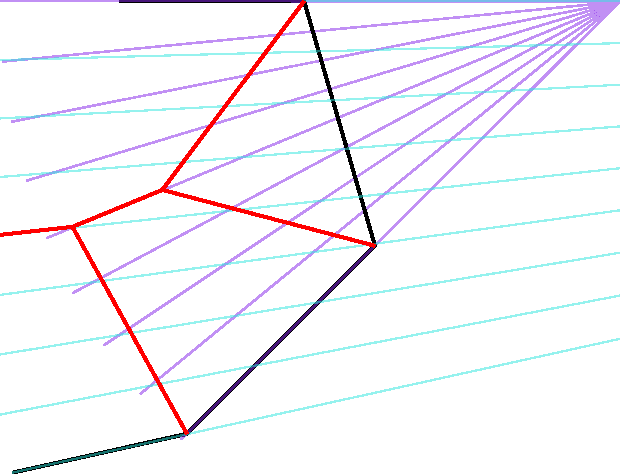
\includegraphics[width=.9\columnwidth]{sources/method/angular_based_spacing.pdf}
\caption{Angular based spacing isn't feasible. The bottom medial axis bone has different spacing based on the two patches. The radially evenly spaced lines are drawn in cyan for the interaction between the bottom outline segment with the top segment and in purple for the interaction between the second bottom segment with  the top segment.}
\label{angular_based_spacing}
\end{figure}



\subsection{Angle of fingers introduced on the skeleton}
\Cref{finger_angles}
Cannot be optimized.
Always has to be orthogonal to the polygon segment.
Otherwise the algorithm isn't stable w.r.t. extra vertices.

\begin{figure}[H]
\begin{subfigure}{0.45\columnwidth}
\includegraphics[width=\columnwidth]{sources/method/finger_angles.jpg}
\caption{Stability against extra vertices}
\label{finger_angles_stability}
\end{subfigure}
\begin{subfigure}{0.45\columnwidth}
\includegraphics[width=\columnwidth]{sources/method/finger_angles_2.jpg}
\end{subfigure}
\caption{Figner angles should always be orthogonal to the outlines}
\label{finger_angles}
\end{figure}



\subsection{Single bead segments}
\Cref{single_bead_strategy}
Could be printed from polygon and return to polygon over same segment without extruding

How to deal with single beads connecting two polys?
: Print 1st poly $\to$ print single bead $\to$ print 2nd poly $\to$ travel over single bead $\to$ print 1st poly

How to deal with three-way intersection single beads?
: Cut up in 1 single bead connecting two polys and 1 normal single bead only connected to one poly

\begin{figure}[H]
\begin{subfigure}{0.45\columnwidth}
\includegraphics[width=\columnwidth]{sources/method/single_bead_strategy.jpg}
\caption{Overview}
\label{single_bead_strategy_overview}
\end{subfigure}
\begin{subfigure}{0.45\columnwidth}
\includegraphics[width=\columnwidth]{sources/method/single_bead_strategy_order.jpg}
\caption{Travel order}
\end{subfigure}
\caption{We can do single-bead segments. Blue is travel move.}
\label{single_bead_strategy}
\end{figure}


\subsection{When to introduce fingers?}
Depends on the angle between the poly segments

When to introduce joints rather than using existing joints? When round joint distances to integer multiples of the nozzle size rather than introducing a new joint?

\paragraph{We could introduce bones implicitly.}
Instead of changing the straight skeleton and introducing bones,
we can simply introduce new vertices on the polygon and generate a new straight skeleton.



%\subsection{Where to add fingers?}
%\Cref{rounded_dist_measures}
%Based on unrounded distance measures.
%Otherwise we don't get the switch to twice the bead width.
%Moreover, the algorithm wouldn't be stable: the locations where bones would get introduces would depend on where the other joints are, instead of on the distance measure.
%\hl{But what does this mean?
%When should I round distances to integer multiples?!}





\subsection{Angle estimation}
When the angle between two outline segments is small, the naive method will produce long triangular cusps.
We can measure the angle between two outline segments which generate a MAT segment by looking at the angle where the lines going through those segments (would) meet.
Equivalently we can compare the Euclidean distance between two vertices with the difference in distance measure;
if the Euclidean distance is larger than twice the distance measure difference, the angle between the segments is less than {\SI{60}{\degree}}.

\begin{figure}[H]
\centering
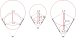
\includegraphics[width=.9\columnwidth]{sources/method/distance_based_angles.pdf}
\caption{Distance based angle estimation. By comparing the euclidean distance between two vertices with the distance measure of the MAT we can skip comparing the angles between the outline segments.}
\label{distance_based_angles}
\end{figure}

The Euclidean distance between two MAT vertices can never be less than the difference in the MAT distance measure between the vertices:t
\begin{figure}[H]
\centering
\includegraphics[width=.3\columnwidth]{sources/method/distance_ratio_limit.pdf}
\caption{Minimal Euclidean distance for a given difference in MAT distance measure.}
\label{distance_ratio_limit}
\end{figure}




\subsection{Determining which parts of the MAT should be transformed}
\Cref{rounded_dist_measures}
\paragraph{line-line-segments}
We mark bones as to-be-transformed based on the angle between the two edges of the polygon for which this bone is the bisector.

\paragraph{line-point segments}
For a parabola MAT segment generated by point $(0,d)$ and an outline segment lying on the x-axis, the parabola is given by $y = \frac{1}{2d} x^2 + \frac12 d$.
The angle between the outline segments is twice the angle between the MAT segment and an outline segment.
The angle between the MAT parabola and the x-axis is the inverse tangent of the derivative of this formula: $\tan^{-1} \left( \abs x / d \right)$.
The angle is less than \SI{60}{\degree} when 
$\tan^{-1} \left( \abs x / d \right) < \SI{30}{\degree}$ 
i.e. when $\abs x/d < 1 / \sqrt{3}$
i.e. when $\abs x < d / \sqrt{3}$.
So we mark the part of the parabola as to-be-transformed for which $x \in [-d / \sqrt{3}, d / \sqrt{3}]$.


\paragraph{point-point segments}
For a segment gerenated by points $(0,0)$ and $(0,d)$, the MAT segment is given by $y=\frac12 d$.
For a given $x$ the distance $D$ to the outline vertices is given by $D = \sqrt{x^2 + \frac12 d}$.
The ratio between MAT distance $D$ and Euclidean distance $\abs x$ is determined by $\frac{\partial D}{\partial x} / \frac{\partial \abs x}{x} = \abs \frac{x}{\sqrt{x^2 + d/2}}$
So the Euclidean distance is more than twice the MAT distance then $\abs \frac{\partial D}{\partial x}  < \frac12$, 
%Wolfram Alpha:
so $\abs x < \frac{\sqrt{d}}{\sqrt{6}} \approx 0.408 d$.
So we mark the part of the straight MAT segment as to-be-transformed for which $x \in [-\frac{\sqrt{d}}{\sqrt{6}}, \frac{\sqrt{d}}{\sqrt{6}}]$.
\hl{But that is very weird in combination with the rule that the ends of marked segments should always be rounded! Isn't it?!}


\subsection{Ends of markings}
For vertices at the end of a sequence of marked MAT segments we need to perform rounding on the MAT distance measure, so as to avoid a gap being generated by toolapths around that vertex.
See bottom of \cref{rounded_vs_unrounded}.

It impossible for three marked edges to come together.
(Simple case) If 2 edges of the MAT meet then 3 outline segments are involved; lines through those segments form a triangle which cannot have more than two angles less than \SI{60}{\degree}.

However, \hl{what if we connect two marked segments using a small segment?}
It seems there is some distance limit based on \cref{distance_ratio_limit}.





\subsection{MAT distance remapping}
In a narrow cusp region we have to transfer from $n$ to $n-1$ beads; this transition requires a distance.
See \cref{single_bead_strategy_overview}.
We use a distance of the median bead width for the transition.
The transition needs to be robust against extra fingers in the MAT
How do we compute the vertex location of an inset on a finger which crosses a transitional segment in the middle?

By aligning the MAT distance with Euclidean space around the transition locations, we obtain a stable method for determining the vertex locations of insets.
See \cref{distance_rounding_transition}.
The extra fingers (blue) cause a negligible difference in the inset path (compare the black dashed pat hwith the red dashed path).

\begin{figure}[H]
\centering
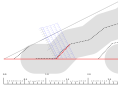
\includegraphics[width=.9\columnwidth]{sources/method/distance_rounding_transition.pdf}
\caption{MAT distance remapping.}
\label{distance_rounding_transition}
\end{figure}





\subsection{Where to round distance measures?}
When a vertex in the medial axis has only a part of the connected bones marked then the distance measure should be rounded?
But that isn't stable against perturbations such as \cref{finger_angles_stability}!


\begin{figure}[H]
\centering
\includegraphics[width=.6\columnwidth]{sources/method/rounded_dist_measures.jpg}
\caption{Distance measure rounding}
\label{rounded_dist_measures}
\end{figure}

\begin{figure}[H]
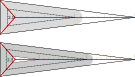
\includegraphics[width=\columnwidth]{sources/method/rounded_vs_unrounded.pdf}
\caption{Toolpaths employing dist rounding vs without.}
\label{rounded_vs_unrounded}
\end{figure}






















